\documentclass[12pt]{article}
\usepackage{amsmath, amssymb, graphics, setspace, breqn, graphicx}
\title{Fonction de Green}
\author{DAVY Leo, KAOUAH Mohammed, ABRIBAT Clement}

\begin{document}
\maketitle
\section{Photo-\'emission et fonction de Green}

Afin de sonder la mati\`ere une m\'ethode exp\'erimentale tr\`es efficace est la spectrom\'etrie.
Cependant la pr\'ediction th\'eorique des spectres est tr\`es difficile \`a calculer. En effet
 les bandes que l'on peut observer sur un spectre correspondent \`a un aper\c cu des niveaux d'\'energie de 
 l'ensemble des particules qui composent la mati\`ere \'etudi\'ee. Or la mati\`ere \'etant compos\'ee de particules fondamentales
  dont on connait les lois qui les r\'egissent d'une mani\`ere tr\`es efficace, ces lois correspondent au mod\`ele standard de la physique des particules.
  Le mod\`ele standard de la physique des particules correspond au regroupement de l'\'electrodynamique quantique, l'int\'eraction faible,
   l'int\'eraction \'electrofaible et la chromodynamique quantique ( int\'eraction forte ).
   \newline
   En l'\'etat de la physique il semble donc que l'on puisse pr\'edire un spectre de photo\'emission. 
   On pourrait donc calculer la fonction d'onde suivante qui int\'eragit avec $N$ particules :
   \begin{equation}
    \Psi(\vec{r_1}, \vec{r_2}, ..., \vec{r_N})
   \end{equation}
    Cependant dans la mati\`ere on a $N \sim 10^{23}$ qui est un nombre tr\`es grand avec lequel on aurait beaucoup de mal
    \`a faire des calculs. Il apparait donc n\'ec\'essaire de trouver une autre mani\`ere de pr\'edire un spectre de photo\'emission.
\subsection{Bases de la photo\'emission}
Nous nous int\'eressons ici \`a la photo\'emission et \`a la photo\'emission inverse.
Il s'agit de deux ph\'enom`enes physiques qui sont li\'es \`a l'int\'eraction entre la mati\`ere
et la lumi\`ere.
\newline
On peut se repr\'esenter la photo\'emission comme \'etant un photon qui est envoy\'e dans de la mati\`ere,
cette mati\`ere va donc \'ejecter un \'electron. La photo\'emission inverse est tr\`es similaire, elle correspond \`a
un \'electron qui est envoy\'e dans de la mati\`ere puis un photon est \'emis depuis cette mati\`ere.
\newline
L'int\'er\^et de la photo\'emission et de la photo\'emission inverse est que les photons ou \'el\'ectrons
\'emis par la mati\'ere pourront \^etre mesur\'es. Les mesures de ces photons ou \'electrons nous renseigneront donc directement
gr\^ace aux relations de la physique quantique, par exemple le fait que les paquets d'\'energie soient quantifi\'es de mani\`ere fixe,
en connaissant l'\'energie des photons ou \'electrons \'emis on peut directement d\'eduire les niveaux d'\'energie des particules de la mati\`ere sond\'ee.

\subsection{\'Etude br\`eve de l'expression formelle de la fonction de Green}
Toutes les \'equations suivantes seront \'ecrites dans le syst\`eme d'unit\'e atomique.
\begin{equation}
 \hbar = m = \frac{e^2}{4 \pi \epsilon_0} = 1
\end{equation}
On peut \'ecrire l'\'equation de Green de la mani\`ere suivante:
/newline
Psi étant trop compliqué à calculer on ne vas pas utiliser cette forme.
\begin{equation}
\label{kamoulox}
 \langle \Psi_0 | T \Psi_H (r_1, t_1) \Psi_H (r_2, t_2) | \Psi_0 \rangle = G(\vec{r_1} t_1, \vec{r_2}  t_2)
\end{equation}
Avec $T$ la ``time-ordering function'' d\'efinie comme suit :
\begin{equation}
 T{A(r_1)B(r_2)} := \theta(t_1 - t_2)A(r_1)B(r_2) \pm \theta(t_2 - t_1)B(r_2) A(R_1)
\end{equation}
Avec $\theta$ la fonction de Heaviside d\'efinie comme suit :

\begin{equation}
\theta(t) = 
\left\{ \begin{array}{rl}
 0 &\ \text{si }x <0\\
 1 &\ \text{si }x \geq 0

\end{array} \right.
\end{equation}
Or les op\'erateurs $\Psi$ de l'\'equation \ref{kamoulox} \'etant trop compliqu\'es \`a calculer dans des syst\`emes r\'eels il est n\'ec\'essaires de simplifier la fonction de Green.
Nous allons donc essayer de la simplifier tout en essayant de conserver un maximum de pr\'ecision dans le reste de ce rapport.
\section{Introduction \`a l'equation de Dyson}
La fonction de Green peut \^etre \'ecrite \`a l'aide de l'\'equation de Dyson. 
\begin{equation}
	G = G_0 + G_0 \Sigma[G] G
\end{equation}
Avec $G$ la fonction de Green qui repr\'esente le syst\`eme, $G_0$ le syst\`eme a l'\'etat initial qui est mesur\'e, et $\Sigma$ une fonctionnelle qui correspond a l'\'energie propre du syst\`eme.
$\Sigma$ s'\'ecrit :
\begin{equation}
	\Sigma[G] = \Sigma_{Hartree}[G] + \Sigma_{XC}[G]
\end{equation}
\begin{equation}
	\Sigma_{Hartree}[G] = \int \rho(r) \frac{1}{\mid r - r'\mid }\mathrm{d}r' 
\end{equation}
avec $v_c$ qui correspond au potentiel coulombien, $\rho(r)$ correspond a la densit\'e \'electronique, et $r-r'$
qui correspond à l'int\'eraction coulombienne.
\begin{equation}
	v_c =  \frac{1}{\mid r - r'\mid }
\end{equation}
\begin{equation}
	\Sigma_{XC} = G \Gamma[G] v_c
\end{equation}
\begin{equation}
	\Gamma[G] = 1 + G^2 \frac{\mathrm{d} \Sigma_{XC}[G]}{\mathrm{d}G} \Gamma[G]
\end{equation}
Cependant ces \'equations dependant de fonctionnelles de G elles sont trop compliqu\'ees \`a r\'esoudre. 
Nous allons donc \'etudier le syst\`eme en dimension spatio-temporelle nulle, c'est \`a dire dans un point, et renommer les variables comme suit
pour plus de clart\'e.
\begin{equation}
	\Sigma \longrightarrow S
\end{equation}
\begin{equation}
	G \longrightarrow y
\end{equation}
\begin{equation}
	\Gamma \longrightarrow g
\end{equation}
\begin{equation}
	v_c \longrightarrow u
\end{equation}
\section{Dyson}
Dans cette section nous allons \'etudier les solutions de l'\'equation suivante en fonction de $g(y)$
\begin{equation}
\label{dyson}
	y = y_0 + y_0 S(y) y
\end{equation}
\subsection{\'Etude de l'\'equation de Dyson avec $g^0(y)$}
On d\'efinit :
\begin{equation}
 g^0(y) = 1
\end{equation}
D'o\`u:
\begin{equation}
 S(y) = S_{XC}(y) + S_{Hartree}(y)
\end{equation}
\begin{equation}
 S_{Hartree}(y) = -uy
\end{equation}
\begin{equation}
 S_{XC}(y) = \frac{1}{2} u y g^0(y) = \frac{1}{2} u y
\end{equation}
\ref{dyson} devient donc :
\begin{equation}
 y = y_0 + y_0 (\frac{-1}{2} u y) y
\end{equation}
\begin{equation}
 y = y_0 - y_0 \frac{1}{2} u y^2
\end{equation}
Il suffit donc de r\'esoudre une \'equation du degr\'e 2.
\begin{equation}
 \Delta = 1 + 2 u y_0^2
\end{equation}
On \`a donc $\Delta > 0 $, on obtient donc les deux solutions suivantes.
\begin{equation}
 y_1 = \frac{1 + \sqrt{1 + 2 u y_0 ^2}}{- u y_0}
\end{equation}
Et 
\begin{equation}
 y_2 = \frac{1 - \sqrt{1 + 2 u y_0^2}}{- u y_0}
\end{equation}
On peut r\'e\'ecrire les solutions pr\'ecedentes de la mani\`eresuivante:
\begin{equation}
 y_1/y_0 = Y_1 = \frac{-1-\sqrt{1 + 2 V}}{V}
\end{equation}
Et 
\begin{equation}
 y_2/y_0 = Y_2 = \frac{-1 + \sqrt{1 + 2V}}{V}
\end{equation}
Avec $V = uy_0^2$. Cependant une seul de ces solutions correspond \`a une solution physique. 
Afin de l'identifier on fait tendre l'int\'eraction Coulombienne vers 0, donc $V\rightarrow 0$ et on fait un d\'eveloppement limit\'e \`a l'ordre 1 de la racine carr\'ee. Ce qui correspond au d\'eveloppementlimit\'e suivant avec a = $\frac{1}{2}$
\begin{equation}
 (1 + x)^a = 1 + ax 
\end{equation}
On obtient donc 
\begin{equation}
 Y_1 = \frac{-1 -1 - \frac{1}{2} 2 V }{V} =\frac{-2 -V}{V}
\end{equation}
\begin{equation}
 Y_2 = \frac{-1 + 1 +\frac{1}{2}2V }{V} = \frac{V}{V} = 1
\end{equation}
Or, lorsque l'on fait tendre le potentiel Coulombien vers 0, c'est \`a dire que les \'electrons n'interagissent plus entre eux, alors ajouter ou enlever un \'electron au syst\`eme ne va pas modifier le syst\`eme. Donc on \`a $y_0 = y$, c'est à dire, $\frac{y_2}{y_0} = 1$.
On peut donc conclure que la solution physique de l'\'equation de Dyson est $Y_2$ lorsque $g^0(y) = 1$.
\newline
Cependant consid\'erer $g^0(y) = 1$ est une approximation, on va donc essayer de r\'esoudre l'\'equation de Dyson de mani\`ere plus pr\'ecise dans la section suivante

\subsection{R\'esolution de l'\'equation de Dyson avec $g^1(y)$}
On consid\`ere dans cette section que 


\begin{equation}
\label{sigma}
	S(y) = S_{XC}(y) + S_{Hartree}(y)
\end{equation}
\begin{equation}
\label{Hartree} 
	S_{Hartree}(y) = -uy
\end{equation}
On \'etudie dans un premier temps $S_{XC}(y)$ 
\begin{equation}
\label{XC} 
	S_{XC}(y) = \frac{1}{2} u y g(y)
\end{equation}
Avec
\begin{equation} 
\label{gamma} 
	g^1(y) = 1 + y^2 \frac{dS_{XC}(y)}{dy} 
\end{equation}
On combine les \'equations \ref{XC} et \ref{gamma} : 
\begin{equation} 
\label{XC_dev}
	S_{XC}(y) = \frac{1}{2} u y (1 + y^2 \frac{dS_{XC}(y)}{dy})
\end{equation}
\begin{equation} 
\label{XC_prime} 
	\frac{dS_{XC}(y)}{dy} = \frac{d(\frac{1}{2} u y )}{y} = \frac{1}{2} u 
\end{equation}
Or $g(y_0) = 1$ ,donc on combine maintenant les \'equations \ref{XC_dev}  et \ref{XC_prime}.
\begin{equation}
\label{XC_final} 
	S_{XC}(y) = \frac{1}{2} u y + \frac{1}{4} u^2 y^3 
\end{equation}
On obtient donc avec \ref{sigma}: 
\begin{equation}
\label{Sigma_final} 
	S(y) = -uy +  \frac{1}{2} u y + \frac{1}{4} u^2 y^3 
\end{equation}
Finalement, on obtient l'\'equation suivante que l'on va chercher \`a simplifier afin de la r\'esoudre.
\begin{equation}
	y = -\frac{1}{2} u y_0 y^2 + \frac{1}{4} u^2 y_0 y^4 + y_0
\end{equation}
\begin{equation}
	\frac{1}{4} u^2 y_0 y^4 -\frac{1}{2} u y_0 y^2 - y + y_0 = 0
\end{equation}
On multiplie l'\'equation pr\'ecedente par $$ \frac{4}{u^2 y_0}$$
On obtient : 
\begin{equation}
	y^4 -\frac{2}{u} y^2 - \frac{4y}{y_0  u^2} + \frac{4}{u^2} = 0
\end{equation}
Posons $$ U = \frac{2}{u}$$
\begin{equation}
\label{Dyson_final} 
	y^4 - U y^2 - U^2\frac{y}{y_0} + U^2 = 0
\end{equation}
Il faut donc maintenant r\'esoudre \ref{Dyson_final}
%
Afin de résoudre cette \'equation de degr\'e 4 nous allons utiliser la m\'ethode de Lagrange.
\section{R\'esolution de l'\'equation de Dyson}
\subsection{R\'esolution avec la m\'ethode g\'en\'erale nouvelle version}

\begin{equation}
\label{YFinal}
 \frac{1}{4} V ^2 Y^4 - \frac{1}{2} V Y^2 -Y + 1 = 0
\end{equation}
Avec 
\begin{equation}
 V = u y_0^2
\end{equation}
Et 
\begin{equation}
 Y = \frac{y}{y_0}
\end{equation}

L'\'equation \ref{YFinal} peut s'\'ecrire :
\begin{equation}
 a y^4 + b y^3 + c y^2 + d y + e = 0
\end{equation}
Avec $a = \frac{1}{4}V^2$,$b = 0$, $c=\frac{-1}{2}V$, $d = -1$, $e=1$ .
\newline
On va donc calculer $\Delta$ afin d'identifier la forme des solutions.
\begin{align*}
\label{Delta}
 \Delta = 256a^3 e^3 - 192 a^2bde^2 - 128 a^2 c^2 e^2 + 144a^2cd^2e - 27a^2d^4\\ 
 + 144 ab^2ce^2 - 6ab^2d^2e - 80abc^2de + 18abcd^3 + 16ac^4e\\
 -4ac^3d^2-27b^4e^2+18b^3cde - 4b^3d^3 - 4b^2c^3e+b^2c^2d^2
 \end{align*}
\begin{equation}
 \Delta = 256a^3 e^3 - 128 a^2 c^2 e^2 + 144a^2cd^2e - 27a^2d^4 + 16ac^4e -4ac^3d^2
\end{equation}

\begin{equation}
 \Delta = 2V^6 - 5V^5 - \frac{27}{16} V^4 + \frac{1}{8}V^6
\end{equation}
\begin{equation}
\label{P}
 P = 8ac - 3b^2 = -V^3
\end{equation}
\begin{equation}
 \Delta_0 = c^2-3bd + 12ae = \frac{13}{4}V^2
\end{equation}
\begin{equation}
 D = 64a^3e -16a^2c^2 + 16ab^2c - 16a^2bd -3b^4
\end{equation}
\begin{equation}
\label{D}
 D = V^6
\end{equation}
On fait l'hypoth\`ese que $\Delta > 0$ et d'apr\`es \ref{P} et \ref{D} on \`a $ D>0$ et $P>0$.
On en d\'eduit donc qu'il y a deux paires de racines complexes conjugu\'ees non r\'eelles.

\begin{equation}
 p = \frac{8ac - 3b^2}{8a^2} = \frac{-2}{V}
\end{equation}
\begin{equation}
 q = \frac{b^3 - 4abc + 8a^2d}{8a^3} = \frac{-4}{V^2}
\end{equation}

On obtient ensuite 
\begin{equation}
S = \frac{1}{2} \sqrt{\frac{-2}{3}p + \frac{1}{3}(Q + \frac{\Delta_0}{Q})}
\end{equation}
O\`u :
\begin{equation}
\label{Q}
Q = \sqrt[3]{\frac{\Delta_1 + \sqrt{\Delta_1^2 - 4 \Delta_0^3}}{2}}
\end{equation}
Avec :
\begin{equation}
 \Delta_1 = 2c^3 - 9bcd + 27b^2e + 27ad^2 - 72ace = \frac{V^2}{4}(-V+27+36V) 
\end{equation}
\begin{equation}
 \Delta_1 = \frac{V^2}{4}(35V +27)
\end{equation}

Or
\begin{equation}
 \Delta_1^2-4\Delta_0^3 = - 27\Delta
\end{equation}
On peut donc \'ecrire \ref{Q}
\begin{equation}
Q =  \sqrt[3]{\frac{\Delta_1+\sqrt{-27\Delta}}{2}}
\end{equation}
\begin{equation}
 Q = \frac{1}{\sqrt[3]{2}}\sqrt[3]{V^2(\frac{V^6}{16}(35V^2+70*27*V+27^2) + \sqrt{-27(2V^2 -5V - \frac{27}{16} + \frac{1}{8}V^2)})}
\end{equation}


\begin{equation}
 S = \frac{1}{2}\sqrt{\frac{4}{3V} + \frac{1}{3}(Q + \frac{\Delta_0}{Q}) }
\end{equation}
Finalement on obtient les diff\'erentes racines :
\begin{equation}
 y_{1,2,3,4} = \pm S \pm \frac{1}{2}\sqrt{-4S^2-2p+\frac{q}{S}}
\end{equation}
\begin{equation}
 y_{1,2,3,4} = \pm S \pm \frac{1}{2}\sqrt{-4S^2+\frac{4}{V}-\frac{4}{V^2 S}}
\end{equation}
\begin{equation}
\left\{ \begin{array}{rl}
y_{1} = - S - \frac{1}{2}\sqrt{-4S^2+\frac{4}{V}-\frac{4}{V^2 S}}\\
y_{2} = - S + \frac{1}{2}\sqrt{-4S^2+\frac{4}{V}-\frac{4}{V^2 S}}\\
y_{3} = + S - \frac{1}{2}\sqrt{-4S^2+\frac{4}{V}-\frac{4}{V^2 S}}\\
y_{4} = + S + \frac{1}{2}\sqrt{-4S^2+\frac{4}{V}-\frac{4}{V^2 S}}
\end{array} \right.
\end{equation} 

\subsection{R\'esolution avec Mathematica}
 
Dans cette partie nous allons nous \'etudier la fonction de Green \`a l'aide du logiciel de calcul formel Mathematica.
Tout d'abord nous pouvons v\'erifier les racines obtenues pr\'ecedemment pour l'\'equation \ref{YFinal}. Nous obtenons ainsi les r\'esultats suivants :
\begin{dmath}
Y_{1,2,3,4} \pm\frac{1}{2} \left(\frac{4}{3 V}+\frac{26}{3 \left(27 V^2+35 V^3+3 \sqrt{3} \sqrt{27 V^4+70 V^5-36 V^6}\right)^{1/3}}+\frac{2
\left(27 V^2+35 V^3+3 \sqrt{3} \sqrt{27 V^4+70 V^5-36 V^6}\right)^{1/3}}{3 V^2}\right)^{\frac{1}{2}} \newline
\pm\frac{1}{2} \left(\frac{8}{3 V}-\frac{26}{3 \left(27 V^2+35 V^3+3
\sqrt{3} \sqrt{27 V^4+70 V^5-36 V^6}\right)^{1/3}}
\newline
-\frac{2 \left(27 V^2+35 V^3+3 \sqrt{3} \sqrt{27 V^4+70 V^5-36 V^6}\right)^{1/3}}{3 V^2}-
\newline
\frac{8}{V^2
\sqrt{\frac{4}{3 V}+\frac{26}{3 \left(27 V^2+35 V^3+3 \sqrt{3} \sqrt{27 V^4+70 V^5-36 V^6}\right)^{1/3}}+\frac{2 \left(27 V^2+35 V^3+3 \sqrt{3} \sqrt{27
V^4+70 V^5-36 V^6}\right)^{1/3}}{3 V^2}}}\right)^{\frac{1}{2}}
\end{dmath}
 Ces r\'esultats correspondent bien \`a ceux obtenus pr\'ecedemment nous allons donc chercher \'a obtenir la ( ou les ) solution(s) physiques.
Nous allons proc\'eder de la m\^eme mani\`ere que avec $g^0(y)$. En effet nos racines correspondent \`a $Y = \frac{y}{y_0}$ donc lorsque
le potentiel coulombien tend vers 0 alorson devrait avoir $Y\rightarrow1$.
En calculant les limites \`a l'aide de Mathematica nous obtenons les r\'esultats suivant.
\begin{alignat}{2}
lim_{V->0} Y_1 &= - \infty - \infty \imath\\
lim_{V->0} Y_2 &= - \infty + \infty \imath\\
lim_{V->0} Y_3 &= 1\\
lim_{V->0} Y_4 &= + \infty
\end{alignat}
On a donc deux solutions complexes et deux solutions r\'eelles comme on avait pu le d\'eterminer en calculant $\Delta$, $D$ et $P$, ce ne seront donc pas des solutions physiques
\`a dl'\'equation de Dyson. Parmi les solutions r\'eelles on voit que $Y_3$ converge vers 1, c'est donc la solution physique du syst\`eme. 
Afin d'\'etudier les r\'esultats de mani\`ere qualitative (Figure \ref{Sola}) nous allons maintenant \'etudier les repr\'esentations graphique des quatre solutions.

\begin{figure}
\caption{Trac\'e des quatre solutions, $Y_N = f_N(V)$}
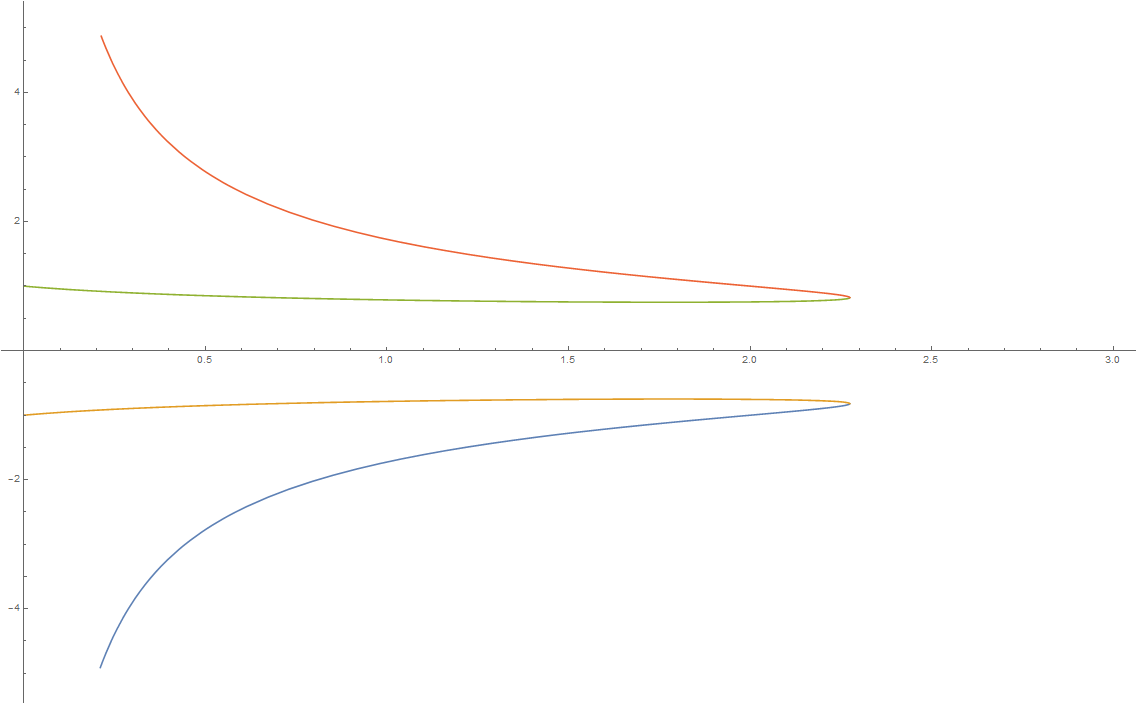
\includegraphics[width = \textwidth]{Courbes4.png}
 \label{Sola}
\end{figure}
 On \`a $S_1$ en bleu, $S_2$ en orange, $S_3$ en vert et $S_4$ en rouge (Figure \ref{Sola}.
 \newline
On observe que les solutions complexes et r\'eelles sont sym\'etriques par rapport \`a l'axe des abscisses.
\begin{figure}
\caption{Trac\'e des deux solutions r\'eelles, $Y_N = f_N(V)$}
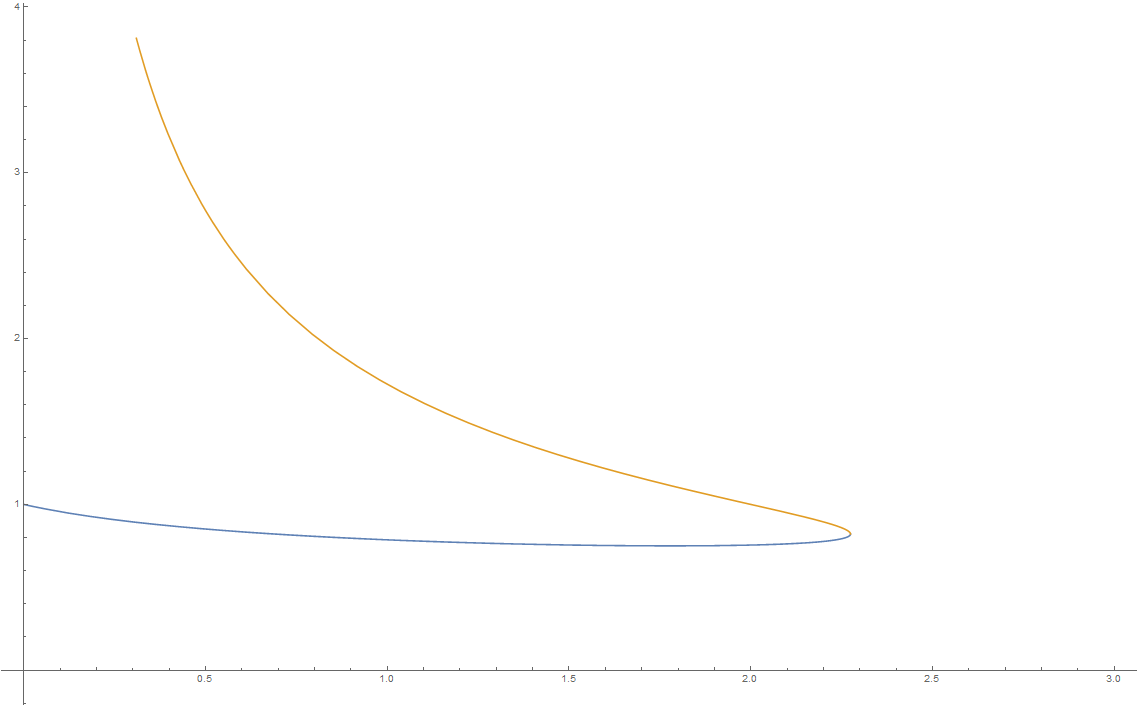
\includegraphics[width = \textwidth]{Courbes2.png}
 \label{Solb}
\end{figure}

Nous allons maintenant nous int\'eresser plus particuli\`erement aux solutions r\'elles (Figure \ref{solb}).
\newline
Nous pouvons ainsi constater que la 
solution physique est quasiment constante et avec une pente faible, alors que la solution non physique a une pente plus importante et diverge en $+\infty$ lorsque
$V\rightarrow0$.












\section{Conclusion}
En nous int\'eressant \`a la fonction de Green dans un point nous avons r\'esolu l'\'equation de Dyson par m\'ethode auto-coh\'erente. 
N\'eanmoins, cette m\'ethode pr\'esente de nombreux inconv\'enients car comme nous l'avons remarqu\'e 
nous ne faisons que nous rapprocher de la solution exacte de
l'\'equation de Dyson en faisant plusieurs it\'erations, l'\'equation augmentant de degr\'e \`a chaque it\'eration. 
Le probl\`eme est qu'il existe plusieurs solutions et qu'il peut \^etre difficile de d\'eterminer la solution physique. 
Il appara\^it donc n\'ecessaire d'utiliser d'autres m\'ethodes afin d'\'etudier la fonction de Green.










\subsection{R\'esolution avec la m\'ethode g\'en\'erale}

L'\'equation \ref{Dyson_final} peut s'\'ecrire :
\begin{equation}
 a y^4 + b y^3 + c y^2 + d y + e = 0
\end{equation}
Avec $a = 1$,$b = 0$, $c=-U$, $d = \frac{-U^2}{y_0}$, $e=U^2$ .
On va donc calculer $\Delta$ afin d'identifier la forme des solutions.
\begin{align*}
\label{Delta}
 \Delta = 256a^3 e^3 - 192 a^2bde^2 - 128 a^2 c^2 e^2 + 144a^2cd^2e - 27a^2d^4\\ 
 + 144 ab^2ce^2 - 6ab^2d^2e - 80abc^2de + 18abcd^3 + 16ac^4e\\
 -4ac^3d^2-27b^4e^2+18b^3cde - 4b^3d^3 - 4b^2c^3e+b^2c^2d^2
 \end{align*}
\begin{equation}
 \Delta = 256a^3 e^3 - 128 a^2 c^2 e^2 + 144a^2cd^2e - 27a^2d^4 + 16ac^4e -4ac^3d^2
\end{equation}
\begin{equation}
 \Delta = 256 U^6 -128 U^6 - \frac{144U^7}{y_0^2} - 27 \frac{U^8}{y_0^4} + 16 U^6 + 4 \frac{U^7}{y_0^2}
\end{equation}
\begin{equation}
 \Delta = U^6(144 - \frac{144U}{y_0^2} - 27 \frac{U^2}{y_0^4} + 4 \frac{U}{y_0^2})
\end{equation}
\begin{equation}
\label{P}
 P = 8ac - 3b^2 = -8c = 8U
\end{equation}
\begin{equation}
 \Delta_0 = c^2-3bd + 12ae = U^2 +12U^2 = 13 U ^2
\end{equation}
\begin{equation}
 D = 64a^3e -16a^2c^2 + 16ab^2c - 16a^2bd -3b^4
\end{equation}
\begin{equation}
\label{D}
 D = 64U^2 -16 U^2 = 48 U^2
\end{equation}
On fait l'hypoth\`ese que $\Delta > 0$ et d'apr\`es \ref{P} et \ref{D} on \`a $ D>0$ et $P>0$.
On en d\'eduit donc qu'il y a deux paires de racines complexes conjugu\'ees non r\'eelles.

\begin{equation}
 p = \frac{8ac - 3b^2}{8a^2} = c = -U
\end{equation}
\begin{equation}
 q = \frac{b^3 - 4abc + 8a^2d}{8a^3} = d = \frac{-U^2}{y_0}
\end{equation}

On obtient ensuite 
\begin{equation}
S = \frac{1}{2} \sqrt{\frac{-2}{3}p + \frac{1}{3}(Q + \frac{\Delta_0}{Q})}
\end{equation}
O\`u :
\begin{equation}
\label{Q}
Q = \sqrt[3]{\frac{\Delta_1 + \sqrt{\Delta_1^2 - 4 \Delta_0^3}}{2}}
\end{equation}
Avec :
\begin{equation}
 \Delta_1 = 2c^3 - 9bcd + 27b^2e + 27ad^2 - 72ace = -2U^3 + 27\frac{U^4}{y_0^2} + 72U^3 
\end{equation}
Or
\begin{equation}
 \Delta_1^2-4\Delta_0^3 = - 27\Delta
\end{equation}
On peut donc \'ecrire \ref{Q}
\begin{equation}
Q =  \sqrt[3]{\frac{\Delta_1+\sqrt{-27\Delta}}{2}}
\end{equation}
\begin{equation}
Q= \sqrt[3]{\frac{\Delta_1 + U^3\sqrt{-27 *(144 - \frac{144U}{y_0^2} - 27 \frac{U^2}{y_0^4} + 4 \frac{U}{y_0^2})}}{2}} 
\end{equation}
\begin{equation}
 Q= U\sqrt[3]{\frac{-2U + 27\frac{U}{y_0^2} + 72  + \sqrt{-27 *(144 - \frac{140U}{y_0^2} - 27 \frac{U^2}{y_0^4} )}}{2}} 
\end{equation}
\begin{equation}
 S = \frac{1}{2}\sqrt{\frac{2U}{3} + \frac{1}{3}(Q + \frac{\Delta_0}{Q}) }
\end{equation}
Finalement on obtient les diff\'erentes racines :
\begin{equation}
 y_{1,2,3,4} = \pm S \pm \frac{1}{2}\sqrt{-4S^2-2p+\frac{q}{S}}
\end{equation}
\begin{equation}
 y_{1,2,3,4} = \pm S \pm \frac{1}{2}\sqrt{-4S^2+2U-\frac{U^2}{Sy_0}}
\end{equation}
\begin{equation}
\left\{ \begin{array}{rl}
y_{1} = - S - \frac{1}{2}\sqrt{-4S^2+2U-\frac{U^2}{Sy_0}}\\
y_{2} = - S + \frac{1}{2}\sqrt{-4S^2+2U-\frac{U^2}{Sy_0}}\\
y_{3} = + S - \frac{1}{2}\sqrt{-4S^2+2U-\frac{U^2}{Sy_0}}\\
y_{4} = + S + \frac{1}{2}\sqrt{-4S^2+2U-\frac{U^2}{Sy_0}}
\end{array} \right.
\end{equation} 



\subsection{R\'esolution avec la m\'ethode de Lagrange}
Donc \ref{Dyson_final} est de la forme :
\begin{equation}
y^4 + a y^2 + b y + c 
\end{equation}
Avec $$a = -U$$ et $$b = -\frac{U^2}{y_0}$$ et $$c = u^2$$
et on notera $\alpha, \beta, \gamma et \delta$ ses solutions. 
On pose d, e et f les solutions de l'\'equation suivante : 
\begin{equation}
y^3 - a y^2 -4cy - b^2 + 4 ac = 0
\end{equation}
On cherche donc les solutions d'une equation du troisi\'eme degr\'e.
On pose $$y = z - U/3$$
On obtient donc l'\'equation :
\begin{equation}
(z - \frac{U}{3})^3  + U (z - \frac{U}{3})^2 - 4 U ^2(z - \frac{U}{3}) + \frac{U^2}{y_0} - 4U^3 = 0
\end{equation}
\begin{equation}
z^3-z^2U+zU^2 - \frac{U^3}{27}+Uz^2-2\frac{zU^2}{3}+ \frac{U^3}{9} - 4U^2z+\frac{4}{3}U^3+\frac{U^2}{y_0}-4U^3 = 0
\end{equation}

\begin{equation}
\label{deg3}
z^3 - z\frac{11}{3}U^2 - u^3\frac{70}{27}+\frac{U^2}{y_0} = 0 
\end{equation}
On peut \'ecrire \ref{deg3} sous la forme :
\begin{equation}
z^3+pz+q = 0
\end{equation}
Avec $$p = -\frac{11}{3}U^2$$ et $$q = - u^3\frac{70}{27}+\frac{U^2}{y_0} $$
On peut donc poser :
\begin{equation}
z^2+27qz - 27p^3 = 0 
\end{equation}
avec $z_{+}$ et $z_{-}$ les solutions de cette \'equation.
On trouve donc $$\Delta = (27q)^2 + 4*27p^3$$
\begin{equation}
\Delta = \frac{U^5*70^2*y_0^2+ 140*27U^5+27^2U^4}{y_0^2} - 4*11^3U^6 
\end{equation}
On obtient donc :
\begin{equation}
z_+ = \frac{U^3 70 + \frac{27U^2}{y_0} +\sqrt{\Delta}}{2} 
\end{equation}
\begin{equation}
z_- = \frac{U^3 70 + \frac{27U^2}{y_0} -\sqrt{\Delta}}{2}  
\end{equation}
On a aussi
\begin{equation}
 \sqrt{\Delta} = \sqrt{\frac{U^5*70^2*y_0^2+ 140*27U^5+27^2U^4}{y_0^2} - 4*11^3U^6 }
\end{equation}

\begin{equation}
 \sqrt{\Delta} = \frac{U^2}{y_0} \sqrt{U*70^2*y_0^2+ 140*27U+27^2 -4*11^3*U^2*y_0^2} = \frac{U^2}{y_0} \sqrt{A}
\end{equation}

On pose maintenant $k$ (respectivement $l$ ) comme \'etant la racine cubique de $z_+$ ( respectivement $z_-$ ).
 Avec $j = e^{i\frac{2\pi}{3}}$
\begin{equation}
\left\{ \begin{array}{rl}
d = \frac{1}{3} ( k + l + U)\\
e = \frac{1}{3} (kj^2 + lj + U)\\
f = \frac{1}{3} (kj + lj^2 + U)
\end{array} \right.
\end{equation} 


\begin{equation}
\left\{ \begin{array}{rl}
d = \frac{U}{3} ( \sqrt[3]{35+\frac{u}{2y_0}(27 + \sqrt{A})}+\sqrt[3]{35+\frac{u}{2y_0}(27 - \sqrt{A})} + 1)\\
e = \frac{U}{3} (\sqrt[3]{35+\frac{u}{2y_0}(27 + \sqrt{A})} e^{i\frac{4\pi}{3}}  +   \sqrt[3]{35+\frac{u}{2y_0}(27 - \sqrt{A})}e^{i \frac{2\pi}{3}} 
+ e^{i\frac{4\pi}{3}} + e^{i\frac{2\pi}{3}} )\\
f = \frac{U}{3} (\sqrt[3]{35+\frac{u}{2y_0}(27 + \sqrt{A})} e^{i\frac{2\pi}{3}}  +   \sqrt[3]{35+\frac{u}{2y_0}(27 - \sqrt{A})}e^{i \frac{4\pi}{3}} 
+ e^{i\frac{2\pi}{3}} + e^{i\frac{4\pi}{3}} )\\
\end{array} \right.
\end{equation}


\begin{equation}
\left\{ \begin{array}{rl}
d = \frac{U}{3} ( \sqrt[3]{35+\frac{u}{2y_0}(27 + \sqrt{A})}+\sqrt[3]{35+\frac{u}{2y_0}(27 - \sqrt{A})} + 1)\\
e = \frac{U}{3} (((35+\frac{u}{2y_0}(27 + \sqrt{A})) e^{i4\pi})^{\frac{1}{3}} + ((35+\frac{u}{2y_0}(27 - \sqrt{A})))e^{i 2\pi})^{\frac{1}{3}}
+ e^{i\frac{4\pi}{3}} + e^{i\frac{2\pi}{3}} )\\
f = \frac{U}{3} (((35+\frac{u}{2y_0}(27 + \sqrt{A})) e^{i2\pi})^{\frac{1}{3}} + ((35+\frac{u}{2y_0}(27 - \sqrt{A}))e^{i 4\pi})^{\frac{1}{3}} 
+ e^{i\frac{2\pi}{3}} + e^{i\frac{4\pi}{3}} )\\
\end{array} \right.
\end{equation}
Or
\begin{equation}
 e^{i4\pi} = e^{i2\pi} = 1
\end{equation}
Et
\begin{equation}
 j^2+j= e^{i\frac{4\pi}{3}} + e^{i\frac{2\pi}{3}} = -1
\end{equation}

\begin{equation}
\left\{ \begin{array}{rl}
d = \frac{U}{3} ( \sqrt[3]{35+\frac{u}{2y_0}(27 + \sqrt{A})}+\sqrt[3]{35+\frac{u}{2y_0}(27 - \sqrt{A})} + 1)\\
e = f = \frac{U}{3} (\sqrt[3]{(35+\frac{u}{2y_0}(27 + \sqrt{A}))} + \sqrt[3]{(35+\frac{u}{2y_0}(27 - \sqrt{A}))} -1 )\\
\end{array} \right.
\end{equation}
Par ailleurs, on a :
\begin{equation}
\left\{ \begin{array}{rl}
\alpha + \beta + \gamma + \delta = 0 \\
\alpha \beta + \gamma \delta = d \\
\alpha \gamma + \beta \delta = e \\
\alpha \delta + + \beta \gamma = f \\
\end{array} \right.
\Longleftrightarrow
\left\{ \begin{array}{rl}
\alpha + \beta + \gamma + \delta = 0 \\
(\alpha + \beta )( \gamma + \delta ) = e+f \\
(\alpha + \gamma)( \beta + \delta) = d +f \\
(\alpha  + \delta)( \beta + \gamma) = d+e \\
\end{array} \right.
\end{equation}
On d\'eduit ensuite des \'equations de ce syst\`eme :
\newline
$\alpha + \beta = \rho_1$ , $\gamma + \delta = -\rho_1 $ avec $\rho_1 = \sqrt{-e-f} $
\newline
$\alpha + \delta = \rho_2$ , $\beta + \gamma = -\rho_2$ avec $\rho_2 = \sqrt{-d -e}$
\newline
$\alpha + \gamma = \rho_3$ , $\beta + \delta = -\rho_3$ avec $\rho_3 = \sqrt{-d-f}$ 
On a donc : 
\begin{equation}
 \rho_1 = \sqrt{-e-f} = \sqrt{-2e} = \sqrt{\frac{-2U}{3} (\sqrt[3]{(35+\frac{u}{2y_0}(27 + \sqrt{A}))} + \sqrt[3]{(35+\frac{u}{2y_0}(27 - \sqrt{A}))} -1 )}
\end{equation}
\begin{equation}
 \rho_2 = \sqrt{-d-e} = \sqrt{\frac{-2U}{3} (\sqrt[3]{(35+\frac{u}{2y_0}(27 + \sqrt{A}))} + \sqrt[3]{(35+\frac{u}{2y_0}(27 - \sqrt{A})})}
\end{equation}
\begin{equation}
 \rho_3 = \sqrt{-d-f} = \sqrt{-d-e} = \rho_2
\end{equation}
On d\'eduit maintenant:
\begin{equation}
 \alpha = \frac{1}{2}(\rho_1 + \rho_2 + \rho_3) = \frac{1}{2}(\rho_1 + 2\rho_2)
\end{equation}
\begin{equation}
  \beta = \frac{1}{2}(\rho_1 - \rho_2 - \rho_3) = \frac{1}{2}(\rho_1 - 2\rho_2)
\end{equation}
\begin{equation}
 \gamma = \frac{1}{2}(-\rho_1 - \rho_2 + \rho_3) = \frac{1}{2}(-\rho_1)
\end{equation}
\begin{equation}
  \delta = \frac{1}{2}(-\rho_1 + \rho_2 - \rho_3) = \gamma
\end{equation}
On a donc $\alpha , \beta, \gamma,\delta$ qui sont les solutions de \ref{Dyson_final}.



\end{document}    

    Contact GitHub API Training Shop Blog About 

    © 2017 GitHub, Inc. Terms Privacy Security Status Help 

